\documentclass[a4paper,10pt]{scrbook}
\usepackage{etex}
\usepackage[T1]{fontenc}
\usepackage{geometry}
\usepackage[utf8x]{inputenc}
\usepackage[ngerman]{babel}
\usepackage[german,figure,linesnumbered,lined]{algorithm2e}
\usepackage{tikz}
%\usepackage{tkz-fct}
\usepackage{color}
\usepackage{graphics}
\usepackage{graphicx}
\usepackage{amssymb}
\usepackage{amsmath}
\usepackage{listings}
\usepackage{booktabs}
\usepackage{pdfpages}
\usepackage{pgfplots}
\usepackage{float}
\usepackage{latexsym}
\usepackage{longtable}
\usepackage{latexsym}
\usepackage{enumitem}
\usepackage{pstricks}
\usepackage{stmaryrd}
\usepackage{MnSymbol}
\usepackage{array}
\usepackage{linearb}
\usepackage{titlesec}
\usepackage{listings}


%Mehr Raum zwischen subsections
\titlespacing{\section}{0pt}{*4}{*2.5}
\titlespacing{\subsection}{0pt}{*3.5}{*1.5}

% kleine Anpassungen, damit die Seitenbreite überall außer Titel gleich ist.
\setcounter{secnumdepth}{2}
\setlength{\textwidth}{160mm}
\setlength{\textheight}{220mm}
\setlength{\headheight}{3mm}
\evensidemargin1mm
\oddsidemargin1mm

%Schwarze MAgie, Vodoo, ....
\newcommand{\tab}{\hspace*{3em}}
\newcommand{\RM}[1]{\MakeUppercase{\romannumeral #1}}

%Java Anpassungen

\definecolor{javared}{rgb}{0.6,0,0} % for strings
\definecolor{javagreen}{rgb}{0.25,0.5,0.35} % comments
\definecolor{javapurple}{rgb}{0.5,0,0.35} % keywords
\definecolor{javadocblue}{rgb}{0.25,0.35,0.75} % javadoc

\lstset{language=Java,
basicstyle=\ttfamily,
keywordstyle=\color{javapurple}\bfseries,
stringstyle=\color{javared},
commentstyle=\color{javagreen},
morecomment=[s][\color{javadocblue}]{/**}{*/},
numbers=left,
numberstyle=\tiny\color{black},
stepnumber=1,
numbersep=10pt,
tabsize=4,
showspaces=false,
showstringspaces=false}


% Farbanpassung
\newrgbcolor{pgreen}{0 1 0}
\newrgbcolor{pblue}{0 0 1}
\newrgbcolor{plightgrey}{0.3 0.3 0.3}
\newrgbcolor{pgrey}{0.6 0.6 0.6}
\newrgbcolor{pdarkgrey}{0.8 0.8 0.8}
\newrgbcolor{pred}{1 0 0}
\newrgbcolor{pviolet}{1 0 1}

%Subsections werden hiermit nicht in das Inhaltsverzeichnis übernommen
\setcounter{tocdepth}{1}


%Dokumentenanfang mit diversen input von mehreren Einzeldokumenten.
\begin{document}
	\begin{titlepage}
\center
\Large Einführung in die Programmierung WS 12-13\large \\[2em]
Lernskript \\[2em]
Dozent:\\Dr. Hildebrandt\\[2em]
\LaTeX{} von:\\Sven Bamberger\\[2em]
Zuletzt Aktualisiert:\\\today\\

\includegraphics[scale=.2]{front/pics/Logo.jpg}\\\quad\\
\end{titlepage}
 
	
	\frontmatter 
		Dieses Skript wurde erstellt, um sich besser auf die Klausur vorzubereiten.\\
\qquad\\
\qquad\\
\textcolor{red}{\Large{Dieses Dokument garantiert weder Richtigkeit noch Vollständigkeit, da es aus Mitschriften gefertigt wurde und dabei immer Fehler entstehen können. Falls ein Fehler enthalten ist, bitte melden oder selbst korrigieren und neu hoch laden.}}


		 
\tableofcontents 
 
	 
	\mainmatter 
		\chapter{Vorlesungen}
%
%
%
\section{Java-Editionen}
	\begin{itemize}
	\item Java läuft auf sehr unterschiedlichen Systemen
	\item  Wird in verschiedenen „Packungsgrößen“ angeboten
	\begin{itemize}
		\item EE (enterprise edition): große Unternehmensserver
		\item SE (standard edition): Desktop-Systeme
		\item ME (micro edition): Handys, PDAs, Embedded Systems
	\end{itemize}
	\item Editionen unterscheiden sich in den mitgelieferten Zugaben,nicht in der Programmiersprache
	\end{itemize}
%
%
%
\section{Java-Entwicklungssystem}
\begin{itemize}
\item Zum Schreiben neuer Programm ist der Compiler javac nötig, zum Ausführen fertiger Programm nicht
\item  Java für verschiedene Einsatzzwecke:
	\begin {itemize}
		\item JRE (java runtime environment): zum Ausführen fertiger Programme
		\item JDK (java development kit): JRE + Compiler und weitere Hilfsmittel zum Schreiben neuer Programme
	\end{itemize}
\end{itemize}
 %
 %
 %
 \section{Namen in Java}
 \begin{itemize}
 \item An vielen Stellen frei wählbare Namen = „Bezeichner“, „Identifier“
 \item Bestandteile: Große und kleine Buchstaben, Ziffern, Underscore (\_)
 \item Erstes Zeichen darf keine Ziffer sein
 \item Etwa fünfzig reservierte Wörter dürfen nicht als Identifier benutzt werden (beispielsweise class, int, public)
	 \item Beispiele:
 	\begin{itemize}
		\item Counter
		\item colorDepth
		\item Iso9660
		\item XMLProcessor
		\item MAX\_VALUE
	\end{itemize}
	\item Nicht erlaubt sind z.B.:
	\begin{itemize}
		\item1stTry 	(erster Buchstabe darf keine Ziffer sein)
		\item Herz Dame (Leerzeichen im Namen nicht erlaubt)
		\item const (reserviertes Wort)
		\item muenchen-erding (Bindestrich im Namen nicht erlaubt)
	\end{itemize}
	\item Übliche Konventionen für Java-Identifier:
	\begin{itemize}
		\item Variablen, Methoden, primitive Typen: CamelCode, erster Buchstabe klein: counter, find1stToken, bottomUp
 		\item Referenztypen: CamelCode, erster Buchstabe groß: Hello, String, ServerSocket
		\item Typvariablen (Generics): einzelne große Buchstaben: T, U
		\item statische, öffentliche Konstanten: alle Buchstaben groß, Wortteile getrennt mit Underscore: MAX\_VALUE, PI, RGB24
	\end{itemize}
\end{itemize}
%
%
%
\section{Regel Ebenen}
\subsection{Syntax (Rechtschreibung)}
Verteilung von Semikolons, Klammern, Schreibweise von Namen
\subsubsection{Syntaxfehler}
Compiler meldet einen Fehler

\subsection{Semantik (Bedeutung)}
Zulässige Kombination von Sprachelementen
\subsubsection{Semantikfehler}
Compiler meldet einen Fehler, Programm verhält sich falsch, stürzt
nach dem Start ab, ...

\subsection{Pragmatik (Gebrauch)}
Bewährte und sinnvolle Konstruktionen
\subsubsection{Fehler der Pragmatik}
Programm ist unleserlich, umständlich, unverständlich
%
%
%
\section{Polymorphismus}
\begin{itemize}
	\item Der Typ des Ergebnisses, und u.U. der Wert, ist abhängig von
	den Typen der Operanden:
	\begin{description}
		\item []$ 20/8 \rightarrow 2 $
		\item []$20.0/8.0 \rightarrow 2.5$
	\end{description}
	\item Zwei Operanden gleichen Typs: Operandentyp = Ergebnistyp
	\item Gemischte Operandentypen: double-Ergebnis:
	\begin{description}
		\item [] $1 + 2 \rightarrow 3$ (int)
		\item [] $1.0 + 2 \rightarrow 3.0$ (double)
		\item[] $1 + 2.0 \rightarrow 3.0$ (double)
		\item[] $1.0+2.0 \rightarrow 3.0$ (double)
	\end{description}
\end{itemize}
%
%
%
\section{Explizite Typkonversionen}
\begin{itemize}
	\item Hohe Priorität, wie andere unäre Operatoren:
	\begin{description}
		\item [] (int)$2.5*3\rightarrow 2*3 \rightarrow 6$
		\item [] -(int)$2.5 \rightarrow -2$
		\item [] Klammern hilft: (int)$(2.5*3) \rightarrow (\textrm{int})(7.5) \rightarrow 7$
	\end{description}
	\item ACHTUNG STOLPERFALLE
	\begin{description}
		\item[] (int)$1e100 \rightarrow 2147483647$
	\end{description}
	\item Typcasts auf ein Minimum beschränken.
\end{itemize}
%
%
%
\section{Struktogramme}
\begin{itemize}
	\item Elementarbausteine von Struktogrammen: einfache Anweisungen
	\item Formulierung einzelner Anweisungen
	\item Beschreibungs- oder Darstellungsformen für Algorithmen:
	\begin{itemize}
		\item Umgangssprache \\
		Problematisch: Mißverständnisse, Interpretationsmöglichkeiten, 
		Sprachkenntnisse
		\item Quelltext\\
		Nur mit Kennnis einer konkreten Programmiersprache lesbar
		\item Neutrale, abstrakte Form\\
		Brauchbarer Kompromiss
	\end{itemize}
	\item Populär: Struktogramme (=Nassi-Schneiderman-Diagramme)
	\item Früher auch: Flussdiagramme (flow charts), erlauben wirre Konstruktionen
	\item Ziel: Reduktion auf die Idee, die wesentlichen Strukturen
\end{itemize}
\subsection{Umgangssprachlich}
Definiere n als ganze Zahl\\
Gib n den Wert 4\\
Zähle n um 1 hoch\\
Gib n aus\\
\subsection{Pseudocode}
int n\\
n = 4\\
n = n + 1\\
print n\\
\subsection{Nassi-Schneiderman}
\begin{figure} [H]
	\centering 
	\scalebox{0.6}{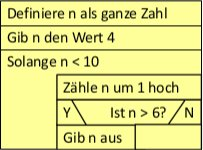
\includegraphics{mainmatter/pics/strukto.jpg}}
	\caption{ein mini Struktogramm} 
\end{figure}
%
%
%
\section{While-Schleife: Euklidischer Algorithmus}
 \begin{lstlisting}[language=JAVA]
class EuclidGCD
{
	public static void main(String... args)
	{
		int m = Integer.parseInt(args[0]);
		int n = Integer.parseInt(args[1]);
		int r = m % n;
		while (r != 0)
		{
			m = n;
			n = r;
			r = m % n;
		}
		System.out.println(n);
	}
}
\end{lstlisting}
%
%
%
\newpage
%
\section{While-Schleife: Collatzfolge (3n + 1 – Folge)}
$z_{n+1} = \left\{ \begin{array}{ll}
         \frac{1}{2}z_{n}, & z_{n}\textrm{ gerade}\\
         3 \cdot z_{n}+1, & z_{n}\textrm{ ungerade}.\end{array} \right. $\\
 \begin{lstlisting}[language=JAVA]
class CollatzMax
{
	public static void main(String... args)	
	{
		int z = Integer.parseInt(args[0]);
		int n = 0;
		int max = z;
		while (z != 1)
		{
			if (z%2 == 0){
				z = z/2;
			}
			else{
				z = 3*z + 1;
			}
			n++;
			if (z > max){
				max = z;
			}
		}
		System.out.println(n);
		System.out.println(max);
	}
}
 \end{lstlisting}
 %
 %
 %
 \section{Inkrement-/Dekrementoperator}
Variable ++; \qquad Variable - -;
 \begin{lstlisting}[language=JAVA]
 int a = 1;
int b = a++; // b = 1, a = 2
int c = a--; // c = 2, a = 1
 \end{lstlisting}
 \qquad\\
++Variable; \qquad - -Variable;
 \begin{lstlisting}[language=JAVA]
int a = 1;
int b = ++a; // b = 2, a = 2
int c = --a; // c = 1, a = 1
 \end{lstlisting}
 %
 %
 %
 \section{Der bedingte Operator}
 \begin{itemize}
 \item Dreistelliger "bedingter Operator" (engl. "conditional operator")
	\item Syntax: \\
		 condition? yes-expression: no-expression
	\item Beziehung zu if:\\
		 variable = condition? yes-expression: no-expression;
	\item äquivalent zu:\\
		 if (condition)\\
		. \qquad variable = yes-expression;\\
		 else\\
		. \qquad variable = no-expression;\\
\end{itemize}
%
%
%
\section{do-while}

\begin{figure} [H]
	\centering 
	\scalebox{0.3}{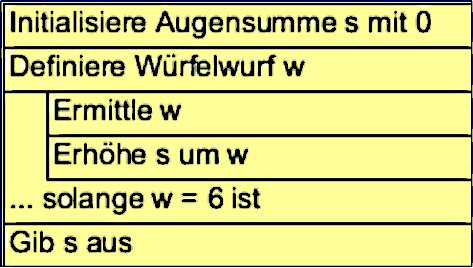
\includegraphics{mainmatter/pics/dowhile.jpg}}
	\caption{ein mini Struktogramm} 
\end{figure}

 \begin{lstlisting}[language=JAVA]
int s = 0;
int w;
do{
	w = // wuerfeln ...
	s += w;
} while (w == 6);
System.out.println(s);
 \end{lstlisting}
%
%
%
\section{Break und Continue}

\subsection{Break}
\begin{itemize}
\item Anweisung break beendet eine Schleife sofort der Rest des Rumpfes wird übersprungen
\item break = einfache Anweisung (wie Definitionen, Wertzuweisungen)
\item Zweck: Entscheidung über Fortsetzung einer Schleife fällt mitten im Rumpf
\end{itemize}

\subsection{continue}
\begin{itemize}
\item Anweisung continue startet sofort den nächsten Schleifendurchlauf der Rest des Rumpfes wird übersprungen
\item Wie break: Nützlich zur Behandlung von Sonderfällen
\item Zweck: Folge von Entscheidungen über Fortsetzung des Schleifendurchlaufes mitten im Rumpf
\end{itemize}	
Achtung: break und continue spalten Kontrollfluss: mit Bedacht
verwenden
%
%
%
\section{Gültigkeitsbereiche}
\begin{itemize}
	\item Idee
	\begin{itemize}
		\item Blöcke {...} gruppieren Anweisungen
		\item Innnerhalb eines Blocks alle Anweisungsarten erlaubt, auch Definitionen
		\item Gültigkeitsbereich (engl. „scope“) einer Variablen...
		\begin{itemize}
			\item beginnt mit der Definition und
			\item endet mit dem Block, in dem die Definition steht
		\end{itemize}
		\item Außerhalb des Blocks: Variable gilt nicht
		\item Gültigkeitsbereiche bezogen auf Quelltext, werden vom Compiler 			
			überprüft
		\item Zur Laufzeit irrelevant
	\end{itemize}
	\item Namenskollision
	\begin{itemize}
		\item Gültigkeitsbereich umfasst untergeordnete (geschachtelte) Blöcke
		\item Namenskollision: Definition des gleichen Namens, wie in einem 	
			umfassenden Block
		\item Java: Doppelte Definition unzulässig
		\item Aber: Kein Problem in disjunkten Blöcken:
	\end{itemize}
\end{itemize}
%
%
%
\section{for-Schleife}
Jede For-Schleife kann durch eine While Schleife ersetzt werden. 
 \begin{lstlisting}[language=JAVA]
for(int i = 0; i < 10; i++)
	System.out.println(i);
 \end{lstlisting}
 %
 %
 %
 \section{Switch}
 \begin{itemize}
 \item Der Wert der expression wird einmal berechnet.
\item Das Ergebnis wird nacheinander mit den labels verglichen, bis zum ersten gleichen Wert.
\item  Die dem label nachfolgenden statements werden ausgeführt, bis zum break;
\item Ziel: switch-Anweisungen ersetzen längere, unübersichtliche if-Kaskaden
\item  Syntax:
\end{itemize}
 \begin{lstlisting}[language=JAVA]
switch (expression)
{
	case label1:
		statement ...
		break;
	case label2:
		statement ...
		break;
	...
}
 \end{lstlisting}
\begin{itemize}
\item switch-Rumpf = Gültigkeitsbereich
\item Definitionen im switch-Rumpf gelten immer, nicht aber Initialisierungen
\item Unübersichtlich: besser keine Definitionen im switch-Rumpf
\item switch ist selbst eine Anweisung\\
$\Rightarrow$ kann in einem übergeordneten switch stehen
\item Nützlich um unregelmäßige Tabellen zu implementieren
\item Typ int als switch-Ausdruck zulässig
\item Nicht zulässig:
\begin{itemize}
	\item double (Test von exakten Werten problematisch ⇒ Rundungsfehler)
	\item boolean (nur zwei Werte)
	\item ...
\end{itemize}
\item Allgemein: ganzzahlige Typen und Aufzählungstypen
\end{itemize}

 \subsection{case-Label}
 \begin{itemize}
\item case-Labels müssen eindeutig sein, doppelte Werte unzulässig
\item case-Labels müssen konstant (vom Compiler berechenbar) sein
\item  Das schließt Literale, Numerale, final-Variablen mit compiler-berechenbarem Wert und konstante Ausdrücke ein.
\item Wenn kein case-Label passt, geschieht nichts (ganzes switch wirkt wie eine leere Anweisung)
\item  Mehrere (verschiedene) case-Labels vor einer Anweisungsfolge sind zulässig
\item default = spezielles case-Label, passt auf alle übrigen Werte
\item default darf nur einmal und nur am Ende genannt werden
\item Jeder switch sollte mit einem default enden
\end{itemize}
 \begin{lstlisting}[language=JAVA]
int a = ...;
final int b = 3;
final double c = b*(b + 1);
switch(a)
{
	case 3:
	case 1 + 2:
		System.out.println("yes");
		break;
		
	case (int)c%(b - 1):
		System.out.println("maybe");
		break;
		
	default:
		System.out.println("no");
		break;
}
 \end{lstlisting}
 
 \subsection{Fall through}
 \begin{itemize}
 \item break beendet switch (zweite Anwendung von break neben Schleifen)
\item Falls break fehlt, wird mit den Anweisungen des nächsten Zweiges fortgefahren (engl. „fall through“)
\item Fall through selten sinnvoll, meistens ein Fehler, immer ein Stolperstein
\item Wenn möglich eher nicht verwenden, Programm eher umschreiben
\end{itemize}
%
%
%
\section{Klassen}
Klassen definieren neue Typen

\subsection{Klassennamen}
\begin{itemize}
\item Klassen sind mit eindeutigen Identifiern benannt
\item In der Regel englische Substantive, erster Buchstabe groß
\item Syntax:
 \end{itemize}
 \begin{lstlisting}[language=JAVA]
class Classname
{
	...
}
 \end{lstlisting}

\begin{itemize}
\item Konventionen:
	\begin{itemize}
	\item Jede Klassendefinition in einer eigenen Quelltextdatei (erzwungen bei öffentlichen Klassen)
	\item Dateiname = Klassenname + Extension .java
	\end{itemize}
\end{itemize}

\subsection{Objektvariablen}
\begin{itemize}
\item Objektvariablen sind Variablen, ebenso wie bisher verwendete Variablen
\item Zur begrifflichen Abgrenzung: bisher benutzte Variablen = lokale Variablen
\item Definitionssyntax von Objektvariablen und lokalen Variablen gleich
\item Aber: Ort der Definition unterschiedlich
\end{itemize}
\begin{tabular}{|c|c|}\hline
Objektvariablen & ... Elemente von Klassen \\ \hline
lokale Variablen & ... Anweisungen in Methoden \\ \hline
\end{tabular}
\begin{itemize}
\item Benennung von Objektvariablen:
	\begin{itemize}
	\item wie lokale Variablen
	\item eindeutig innerhalb einer Klasse
	\end{itemize}
\end{itemize}
\subsubsection{Zugriff}
\begin{itemize}
\item Jedes Objekt enthält die Objektvariablen, die in der Klassendefinition festgelegt sind
\item Objektvariablen eines Objektes können einzeln angesprochen werden: Elementzugriff
\item Objekt an das sich ein Elementzugriff richtet: Zielobjekt
\item Syntax: Zielobjekt.Objektvariable
\end{itemize}
\subsubsection{Umgang}
\begin{itemize}
\item Elementzugriff spricht Objektvariablen innerhalb eines Objektes an
\item Gleiche Verwendung wie lokale Variablen
\item Beispiel: Zähler oder Nenner eines Rational-Objektes ...
\begin{itemize}
\item  in einem Ausdruck verwenden:	int i = 5 - r.numer*3;
\item mit Operatorzuweisung und Inkrementoperator modifizieren:\\
r.numer *= 10;\\
r.numer++;
\item vergleichen: if(r.denom != 0) ...
\item usw...
\end{itemize}
\item Nur Zugriffssyntax zeigt Unterschied zwischen Objektvariablen und
lokalen Variablen
\end{itemize}
\subsubsection{Objektvariablen unterschiedlicher Objekte}
\begin{itemize}
\item Jedes Objekt hat eigene Objektvariablen (das ist der ganze Witz...)
\item Elementzugriff richtet sich an eine Objektvariable innerhalb eines Objektes (des Zielobjektes), andere Objektvariablen des Zielobjektes und Objektvariablen anderer Objekte unberührt
\end{itemize}


\subsection{Referenztypen}
\begin{itemize}
\item Classname = neuer Typ, gleichberechtigt neben primitiven Typen
\item int, double, boolean, char, byte, short, long sowie float sind primitive Typen
\item Primitive Typen sind atomar, Bausteine spielen keine Rolle
\item Gegensatz: Classname ist ein Referenztyp $\rightarrow$ enthält separate Bestandteile, diese können einzeln angesprochen und verarbeitet werden
\item Alle Klassen definieren Referenztypen
\item Auswahl primitiver Typen liegt fest, können nicht neu definiert werden
\item Erster Nutzen von Klassen: bündeln ihre Bestandteile
\end{itemize}

\subsection{Objekte / Instanzen}
\begin{itemize}
\item Klassendefinition $\approx$ Bauplan, Konstruktionsvorschrift, Blaupause
\item Objekte der Klasse müssen explizit geschaffen werden, entstehen nicht von alleine
\item  Objekt = Exemplar, Instanz
\item 1 Klassendefinition — beliebig viele Objekte
\end{itemize}

\subsection{Operator new}
\begin{itemize}
\item Erzeugen eines neuen Objektes = instanziieren (auch „konstruieren“, „allokieren“)
\item Syntaktisch mit Operator new.
\item new produziert aus einer Klassendefinition ein einzelnes, neues Objekt dieser Klasse
\item Mehrere Objekte $\Rightarrow$ mehrere Aufrufe von new
\end{itemize}
 \begin{lstlisting}[language=JAVA]
new Classname();
\end{lstlisting}

\subsection{Methoden}
\begin{itemize}
\item Methoden werden in Klassen definiert, ebenso wie Objektvariablen
\item  Objektvariablen legen Eigenschaften („Attribute“) von Objekten fest, Methoden legen Operationen fest
\item  Anders formuliert: Objektvariablen beschreiben den Aufbau von Objekten, Methoden ihr Verhalten
\item Methoden haben Namen, wie Objektvariablen (Achtung: eigener
Namensraum, Methodennamen und Objektvariablennamen clashen
nicht; aber Doppelbelegung beinahe nie sinnvoll)
\end{itemize}
 \begin{lstlisting}[language=JAVA]
class Rational
{
	int numer;
	int denom;
	
	void print()
	{
	System.out.printf("%d/%d%n", numer, denom);
	}
}
 \end{lstlisting}
 \begin{itemize}
 \item Methodendefinition = Methodenkopf + Methodenrumpf
 \item Klammern im Rumpf sind Pflicht, auch bei einer (oder keiner) Anweisung
 \begin{itemize}
 	\item nicht außerhalb einer Klassendefinition
 	\item nicht innerhalb einer anderen Methodendefinition
\end{itemize}
\item Anzahl, Reihenfolge und Anordnung von Methodendefinitionen in einer Klasse beliebig
\end{itemize}
\subsubsection{Aufruf}
\begin{itemize}
\item Methode wird mit Zielobjekt aufgerufen
\item Ohne Zielobjekt kein Aufruf (Ausnahme: statische Methoden)
\item Methodenaufruf syntaktisch ähnlich zu Elementzugriff: Zielobjekt.Methodenname();
\item Runde Klammern markieren Methodenaufruf, fehlen bei Objektvariablenzugriff
\item Ablauf eines Methodenaufrufs in mehreren Einzelschritten: Call-Sequence
\item Aufrufendes Programm („Aufrufer“, engl. caller) unterbrechen
\begin{itemize}
	\item Werte aller Argumente von links nach rechts berechnen
	\item Parameter erzeugen
	\item Parameter mit Argumentwerten initialisieren
	\item (Aufrufendes Programm („Aufrufer“) unterbrechen)
	\item (Methodenrumpf durchlaufen)
	\item Parameter zerstören
	\item (Aufrufer nach dem Aufruf fortsetzen)
\end{itemize}
\end{itemize}
\subsubsection{Methodenrumpf}
\begin{itemize}
\item Methodenrumpf = Block
\item Gültigkeitsbereich lokaler Definitionen = Methodenrumpf
\item Lebensdauer lokaler Variablen: jeweils ein Aufruf (Gegensatz Objektvariablen: Lebensdauer wie Objekt)
\item Zugriff auf Objektvariablen des eigenen Objektes ohne Angabe eines Zielobjekts
\item Ebenso: Aufruf von Methoden des eigenen Objektes ohne Angabe eines Zielobjektes
\item Methoden erreichen jede Objektvariable der eigene Klasse, unabhängig von der Anordnung der Definitionen
\end{itemize}
\subsubsection{Namenskollision}
\begin{itemize}
\item Namen von lokalen Variablen und Objektvariablen kollidieren nicht
\item Vorteil: Benennung von lokalen Variablen ohne Rücksicht auf Objektvariablen
\item Nachteil: Lokale Definition „verdeckt“ Objektvariable (oft unbeabsichtigt).
\item In der Praxis unproblematisch: Zugriffe auf Objektvariablen sowieso besser auf einzelne Methoden beschränkt (Stichwort: Datenkapselung)
\end{itemize}
\subsubsection{Parameterübergabe}
\begin{itemize}
\item Argumente und Parameter vom Compiler bei jedem Aufruf paarweise abgeglichen
\item Ein Argument pro Parameter erforderlich (zu viele oder zu wenige Argumente: wird nicht übersetzt; Ausnahme: Varargs)
\item Nötig: Typ jedes Arguments kompatibel zum entsprechenden Parameter
\item Beliebig komplizierte Ausdrücke als Argumente zulässig, werden erst ausgerechnet, dann übergeben
\item Verwendung der Parameter im Methodenrumpf: vergleichbar mit automatisch initialisierten lokalen Variablen
\item Parameter = dritte Art von Variablen, neben lokalen Variablen und Objektvariablen
\item Liste von Parametern im Methodenkopf (Komma zwischen je zwei Parametern)
\end{itemize}
%
%
%
\section{Methodenüberladung}
\begin{itemize}
\item Überladen (engl. overloading) = mehrere Methoden mit gleichen Namen, aber unterschiedlichen Parameterlisten
\item Sinnvoll für verwandte Methoden mit ähnlichem Zweck
\item Überladen mit unterschiedlicher Parameteranzahl oder unterschiedlichen Parametertypen oder beidem
\item Namen der Parameter ohne Bedeutung
\end{itemize}

\subsection{Aufruf überladener Methoden}
\begin{itemize}
\item overload resolution = Auswahl einer passenden überladenen Methode zu einer gegebenen Argumentliste — manchmal nicht ganz einfach!
\item Zuerst: Alle in Frage kommenden Kandidaten sammeln, einschließlich der Anwendung impliziter Typkonversionen
\item Unter den Kandidaten die Methode aufrufen, die am genauesten passt
\item Was bedeutet: „passt am genauesten?
\item Eine Methode a „passt genauer“ als eine Methode b, wenn jeder Aufruf von a auch von b, akzeptiert werden würde, aber nicht umgekehrt
\end{itemize}

\subsection{Mehdeutige Aufrufe: Aufrufbeispiele}
\begin{itemize}
	\item Letzter Fall: Zwei Kandidaten
\end{itemize}
\begin{tabular}{lr}
set(double, int) & nach Konversion des ersten Argumentes \\
set(int, double) & nach Konversion des zweiten Argumentes
\end{tabular}
\begin{itemize}
\item Jede der beiden Methoden akzeptiert Aufrufe, die die andere nicht akzeptiert. Keine passt genauer als die andere.
\item Der Aufruf ist mehrdeutig — Fehler
\item Methoden nur mit unterschiedlich vielen Parametern oder mit inkompatiblen Parametertypen überladen
\end{itemize}
%
%
%
\section{Ergebnisrückgabe}
\begin{itemize}
\item Mehrere return-Anweisungen im Rumpf erlaubt
\item Methode kehrt zurück, sobald zur Laufzeit das erste return erreicht wird
\item Statische Reihenfolge der return-Anweisungen unerheblich, konkreter Ablauf zur Laufzeit entscheidet
\end{itemize}

\subsection{Idee}
\begin{itemize}
\item Parameterübergabe transportiert Information vom Aufrufer zur Methode
\item Ergebnisrückgabe liefert Information von der Methode zurück zum Aufrufer
\item Eine Methode kann beliebig viele Parameterwerte annehmen, aber nur einen Ergebniswert liefern
\end{itemize}

\subsection{Definition}
Zwei gekoppelte Maßnahmen zur Ergebnisrückgabe:
\begin{itemize}
\item Typ des Ergebniswertes im Methodenkopf
\item return-Anweisung im Methodenrumpf
\end{itemize}

\subsection{Schema}
 \begin{lstlisting}[language=JAVA]
type methodname(...)
{
	...
	return expression;
}
 \end{lstlisting}
\begin{itemize}
\item Typ von expression in der return-Anweisung kompatibel zu type im Methodenkopf
\item Ausdruck „Methodentyp“ = Typ des Ergebniswertes der Methode
\item Auch kurz: „Typ-Methode“ = Methode die ein Ergebnis des Typs liefert
\end{itemize}
%
%
%
\section{Arrays}
\subsection{Motivation}
\begin{itemize}
\item Arrays (auch „Feld“, „Reihung“) vordefiniert, ohne weitere Maßnahmen verfügbar
\item Werden von praktisch allen Programmiersprachen angeboten
\item Tief in Java verankert, von der JVM intern genutzt
\item Arrays sind Containertypen: Speichern Elemente anderer Typen
\item Elementtyp beliebig, aber gleich für alle Elemente
\item Werte einzelner Elemente austauschbar
\item Anzahl Elemente eines Arrays („Arraylänge“) unveränderlich
\end{itemize}

\subsection{Arraytypen}
\begin{itemize}
\item Arrays = Familie von ähnlichen Typen, kein einzelner Typ
\end{itemize}
\begin{tabular}{l|l}
Elementtyp & Arraytyp \\ \hline
int & int[] \\
boolean & boolean[]\\
char & char[]\\
String & String[]\\
Rational & Rational[] \\
OpenCounter & OpenCounter[] \\
\end{tabular}
\begin{itemize}
\item Arraytypen sind Referenztypen
\item Ein Arraytyp legt keine Länge fest
\item Ein konkretes Exemplar eines Arrays hat eine feste, unveränderliche Länge
\end{itemize}

\subsection{Allokieren}
Erzeugen eines neuen Arrays mit einer bestimmten Anzahl Elemente eines beliebigen typs. \\
Beispiele: Arrays mit 4 bzw. 36 Elementen:
 \begin{lstlisting}[language=JAVA]
int [] a = new int[4]
Rational[] b = new Rational[3*8+12]
\end{lstlisting}
a und b referenzieren Arrays welche mit null initialisiert werden. 
\begin{itemize} 
\item Elementanzahl wird zur Laufzeit beim new-Aufruf festgelegt, kann nachher nicht mehr verändert werden
\item Elemente eines Arrays beim Allokieren automatisch mit Defaultwerten vorbesetzt (ebenso wie Objekt- und Klassenvariablen)
\item Bildhafte Vorstellung: Array = Liste namenloser Variablen, werden gemeinsam definiert, bleiben für die Lebensdauer des Arrays beisammen
\item Erzeugt nur das Array, keine Objekte, ruft keinen Element-Konstruktor auf
\end{itemize}

\subsection{Arrayliterale}
\begin{itemize}
\item Arrayliteral = Konstante eines Arraytyps
\item Allokiert neues Array aus einer Liste vorgegebener Werte
\item Schema:\\
. \qquad new type[] {expression, expression, ..., expression}
\item Länge der Arrays = Anzahl Elemente
\item  Beispiel:\\
new int[] {71, -4, 7220, 0, 238}
\item  Listenelemente = beliebige Ausdrücke, kompatibel zum Elementtyp des Arrays
\item Sinnvoll, wenn Anzahl und Werte von Elementen im Quelltext bekannt
\end{itemize}

\subsection{Elementzugriff}
\begin{itemize}
\item Elemente eines Arrays folgen linear aufeinander
\item Jedes Element hat ganzzahligen Index
\item Index des ersten Elementes = 0, dann fortlaufend weiter
\item Index des letzten Elementes = (Arraylänge − 1)
\item Zugriff auf alle Element (ungefähr) gleich schnell = random access
\item Schema für „Array-Elementzugriff“:\\
.\qquad array[expression]
\item Index zur Laufzeit berechnet aus int-Ausdruck expression
\item Zugriff auf ein Element berührt die anderen Elemente des Arrays nicht
\item Arrayelement benutzbar wie gewöhnliche Variable des Elementtyps
\item Unzulässige Indexwerte werfen ArrayIndexOutOfBoundsException
\item Negativer Index immer unzulässig
\item JVM prüft zur Laufzeit jeden Array-Elementzugriff
\item Anzahl Elemente eines Arrays (konzeptionell) beliebig
\item Erlaubt Arrays mit einem und keinem Element
\item Anzahl Elemente als öffentlich lesbare final-Objektvariable length
\item Zugriff wie Objektvariablen in Objekten:\\
array.length

\end{itemize}

\subsection{Syntax}
\begin{itemize}
\item Eckige Klammern syntaktisch in verschiedenen Kontexten
\item Typangaben:\\
Typ + leere eckige Klammern\\
int[] a;
\item Allokieren eines neuen Arrays:\\
new + Typ + Anzahl Elemente in eckigen Klammern\\
a = new int[5];
\item Array-Literal:\\
new + Typ + leere eckige Klammern + Liste von Elementen\\
a = new int[] {1, 2, 3};
\item Elementzugriff:\\
Arrayausdruck + Index in eckigen Klammern\\
a[1] = 23;
\end{itemize}

\subsection{forech-Schleife}
Kurzform einer for-Schleife für bestimmten Zweck\\
for (type variable: array)\\
statement\\
 \begin{lstlisting}[language=JAVA]
 for (int e: a){
 	...
}
\end{lstlisting}
Äquivalent zu:
 \begin{lstlisting}[language=JAVA]
for (int i = 0; i < a.length; i++){
	int e = a[i];
	...
}

\end{lstlisting}
\begin{itemize}
\item Nur Lesen, kein Schreiben des Arrays
\item Start immer mit erstem Element
\item Sequentieller Durchlauf, keine Sprünge
\item Nur ein Array, nicht mehrere parallel
\item Durchlauf abbrechen nur mit break
\end{itemize}
%		\input{mainmatter/chapter_2} 
%		\input{mainmatter/chapter_3} 
	 
	\backmatter 
		\listoffigures 
\end {document}